\ifx\wholebook\relax \else

\documentclass[b5paper]{article}
\usepackage[nomarginpar
  %, margin=.5in
]{geometry}

\addtolength{\oddsidemargin}{-0.05in}
\addtolength{\evensidemargin}{-0.05in}
\addtolength{\textwidth}{0.1in}

\usepackage[en]{../prelude}

\setcounter{page}{1}

\begin{document}

\title{Zero}

\author{Xinyu LIU
\thanks{{\bfseries Xinyu LIU} \newline
  Email: liuxinyu99@hotmail.com \newline}
  }

\maketitle
\fi

\markboth{Zero}{A tour of numbers}

\ifx\wholebook\relax
\chapter{Zero}
\fi

\epigraph{The truth of Being and of Nothing is accordingly the unity of the two: and this unity is Becoming.}{Hegel {\em Short Logic}}

Despite the history of number is over 5000 years, the history of zero is only about 1200 years. Zero is a new comer. It was originated from India, and was introduced to the west through Arabian. Different from 1, 2, 3, ... zero was created as a placeholder but not a number. It looked like a second level citizen in the kingdom of numbers because zero has no value.

\section{Rejection of zero}
People created zero to express nothing. Indian named it as sunya, which meant vacant in Sanskirt. For example, the 0 in number 2025 means there is {\em no} value of hundred. 0 indicates void, which gives negative meaning in the tradition of west (cultural, philosophical, and religious). It was connected with darkness, ending, and death. While 1 means being, there is a thing; 2 means there are two things... One says there is no apple, but not say there is zero apple. In such way, it emphasizes the negate of being. Shakespeare wrote `To be or not to be, that is the question.'

\index{Roman abacus}
\begin{figure}[htbp]
 \centering
 \includegraphics[scale=0.35]{img/Roman-abacus}
 \caption{A bronze Roman abacus in 1st century. There are counting beads in the grooves; each groove represents Roman unit I, V, X, C, and M\cite{Cartwright-2013} (Archaeological Museum, Aosta, Italy).}
 \label{fig:roman-abacus}
\end{figure}

Although seen the big advantage of Hindu-Arabic numeral system in computation, the European people converted the result to Roman numbers in order to avoid zero\footnote{Similarly, Chinese people left empty positions for zero when computing with the counting rods (see \cref{sec:counting-rods}), but they converted the result to the number in multiplicative grouping system, such as a hundred, two thousand and fifteen, a hundred and two. The dedicated character of zero `零' didn't appear until Song and Yuan dynasty.}. Some people treated 0 evil and only used it privately. Clergies computed in Roman numbers with abacus shown in \cref{fig:roman-abacus} (not the Chinese abacus). This tool is derived from Babylonian tablet. The method is to move/change beads among grooves, then record the result in Roman numbers. As more and more people, particularly merchants and bankers, adopted Hindu-Arabic numerals in practice, a challenge between the two systems happened in the 16th century (as in \cref{fig:hindu-arabic-vs-abacus}). It's not hard to imagine the result, Hindu-Arabic system won. Such challenges repeated several times in the history: Stephenson's Rocket, a pioneering steam-powered locomotive vs. horse\footnote{Invented by British engineers George and Robert Stephenson.} in 1830; IBM Deep blue vs. the world chess champion Garry Kasparov in 1997; Google's Alpha-Go vs. 9-dan Go master Lee Sedol and Ke Jie; Open AI's ChatGPT vs. students in SAT test... Every time a revolutionary thing arising, a challenge happens.

\begin{figure}[htbp]
 \centering
 \includegraphics[scale=0.8]{img/Hindu-arabic-vs-abacus}
 \caption{Engraving of Arithmetica (or the Allegory of Arithmetic) supervising a contest between Boethius, representing written calculation using Hindu-Arabic numbers, and Pythagoras, represented as using a counting board. From Gregor Reisch, {\em Margarita philosophica} in 1503.}
 \label{fig:hindu-arabic-vs-abacus}
 %https://old.maa.org/press/periodicals/convergence/mathematical-treasures-margarita-philosophica-of-gregor-reisch
\end{figure}

The win of Hindu-Arabic system gave 0 `citizenship', legitimate to use. But it's a second class citizen. Why 0 can't be first class citizen as $1, 2, 3, \dotsc$?

\section{To be a number}

What does make 0 different from $1, 2, 3, \dotsc$ preventing it from being a first class citizen? It's the value, or magnitude. The value of 1 is 1, for example, the length of 1cm, the mass of 1 gram, the unit of 1 sheep... the value of 2 represents the length of 2cm, the mass of 2 grams, the units of 2 sheep... But what's the value of 0? It has no value. 0 is a placeholder, but not a number because it has no value\cite{Seife-2000}. 0 is so different that it breaks those rules work well for $1, 2, 3, \dotsc$ for example:

\label{sec:archimedes-axiom}
\begin{enumerate}[1)]
\item Archimedes axiom. A number\footnote{All numbers refer to natural number in this section.} increases when adding to itself. Archimedes treated it as an axiom: for any non-zero $m < n$, there is a time that $m + m + \cdots > n$. \index{Archimedes axiom}

\begin{align*}
1 + 1 &= 2   & 1 + 1 + 1 &= 3 & \dots \\
2 + 2 &= 4   & 2 + 2 + 2 &= 6 & \dots \\
3 + 3 &= 6   & 3 + 3 + 3 &= 9 & \dots \\
\dots &      & \dots     &    &
\end{align*}

But $0 + 0 = 0$ does not increase, $0 + 0 + 0 + \cdots$ will never exceeds any number, such as 1.

\item Product. People recognized product from arranges pebbles (or soldiers) in rectangle. $1 \times 5 = 5$ is a rectangle of 1 row and 5 columns; $2 \times 5 = 10$ is a rectangle of 2 rows and 5 columns; $3 \times 5 = 15$ is a rectangle of 3 rows and 5 columns... but what is $0 \times 5$ for? the rectangle vanishes as shown in \cref{fig:grid-vanish}.

\begin{figure}[htbp]
 \centering
   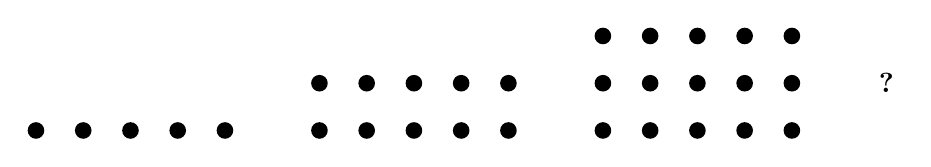
\begin{tikzpicture}[
       scale=0.6,
       dot/.style={circle, fill=black, minimum size=6pt, inner sep=0pt},
       question/.style={font=\Huge, font=\bfseries}
   ]

   \foreach \x in {0,1,2,3,4} {
       \node[dot] at (\x, 0) {};
   }

   \foreach \x in {0,1,2,3,4} {
       \foreach \y in {0,1} {
           \node[dot] at (\x + 6, \y) {};
       }
   }

   \foreach \x in {0,1,2,3,4} {
       \foreach \y in {0,1,2} {
           \node[dot] at (\x + 12, \y) {};
       }
   }

   \node[question] at (18, 1) {?};
   \end{tikzpicture}

 \caption{The rectangle vanishes for $0 \times 5$.}
 \label{fig:grid-vanish}
\end{figure}

\label{sec:mul-as-zoom}
Multiplication means scaling. When scale a ruler 2 times, not only the length of the ruler, but also the length between marks double; when scale 3 times, both the length of the ruler and between marks triple, as shown in \cref{fig:ruler-vanish}. If scale down to $\frac{1}{3}$, then we get a small ruler. But what if scale 0 (times 0)? The ruler together with the marks collapses to a dot; it vanishes.

\begin{figure}[htbp]
 \centering
 \includegraphics[scale=0.35]{img/zoom-rulers}
 \caption{The ruler with marks collapses to a dot without size when scaling 0.}
 \label{fig:ruler-vanish}
\end{figure}

The product represents rectangle; the ruler represents line segment. Multiplication by 0 destroys them. There was no zero in Greek geometry or numeral system. Euclid defined `a point is that which has no parts; a line is length without breadth.' (Definition 1 and 2 in Book I of {\em Elements}.) Is 0 a point?

\item Division is the reverse of multiplication. For example, the reverse of $2 \times 3 = 6$ is $6 \div 2 = 3$; the reverse of $3 \times 4 = 12$ is $12 \div 3 = 4, \dotsc$ the reverse of $2 \times 0 = 0$ is $0 \div 2 = 0$, generally the reverse of $a \times 0 = 0$ is $0 \div a = 0$. However, what would be division by 0?From the reverse of multiplication, $a \div b$ is to find some $c$ satisfying $bc = a$; it means $a \div 0$ is to find some $x$ satisfying $0x = a$. But $0x = 0$, unless $a \ne 0$, there isn't such a $x$, because $0x = 0 \ne a$. Even if $a = 0$ such that the reverse of $0 \times 0 = 0$ looks like $0 \div 0 = 0$, but then the reverse of $1 \times 0 = 0$ will be $0 \div 0 = 1$; the reverse of $2 \times 0 = 0$ will be $0 \div 0 = 2, \dotsc$ any reverse of $a \times 0 = 0$ will be $0 \div 0 = a$, hence $0 \div 0$ can be any number, that is$(0 \div 0) = 0 = 1 = 2 = 3 = \cdots$ Nothing, which is 0, would become being like $1, 2, 3, \dotsc$ Bertrand Russell, in a lecture on logic, mentioned that in the sense of material implication, a false proposition implies any proposition. A student raised his hand and said ``In that case, given that 1 = 0, prove that you are the Pope.'' Russell immediately replied, ``Add 1 to both sides of the equation: then we have 2 = 1. The set containing just me and the Pope has 2 members. But 2 = 1, so it has only 1 member; therefore, I am the Pope.'' \index{0!division by zero}

\begin{align*}
0 = 1 & \Rightarrow 1 = 2     & \text{add 1 to both sides} \\
      & \Rightarrow 1 + 1 = 3 & \text{add 1 to both sides} \\
      & \dotso
\end{align*}

Ian Stewart gives another ridiculous example\cite{Stewart-2019}:

One cat has one tail;

Zero cat has eight tails.

Therefore, adding: One cat has nine tails.
\end{enumerate}

As 0 breaks rules exceptionally, people treat 0 different from $1, 2, 3, \dotsc$. As shown in \cref{fig:keyboard}, 0 comes after numbers 1 to 9.

\begin{figure}[htbp]
 \centering
 \includegraphics[scale=0.35]{img/keyboard}
 \caption{0 in keyboard}
 \label{fig:keyboard}
\end{figure}

\subsection{Ordinal number}
Besides value, number has order. 1 goes first, 2 follows 1, 3 follows 2, and so on. People recognize order from counting. Michael Artin had a conversation with his daughter\cite{MArtin-2011}:

``One, two, three, five, four...''

``No Daddy, it's one, two, three, four, five.''

``Well if I want to say one, two, three, five, four, why can't I?''

``That's not how it goes.''

\begin{center}
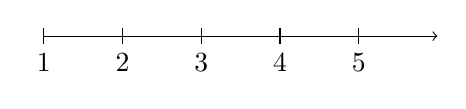
\begin{tikzpicture}
    \draw[->] (-2,0) -- (3,0); % node[right] {$x$};
    \foreach \x in {1,2,3,4,5}
    {
        \draw (\x-3,0.1) -- (\x-3,-0.1) node[below] {$\x$};
    }
    % \draw[fill=black] (-2,0) circle (0.05); % origin
\end{tikzpicture}
\end{center}

\index{number line} \index{ordinal number} \index{dating system}

Arrange numbers in a line, namely the number line. Each number has an order (its ordinality). Our dating system came from an idea of a Christian Monk Dionysius Exiguus in 525 CE. He defined the year that Jesus Christ's birth as {\em Anno Domini}, a Latin term which means Year of our Lord. It was abbreviated as AD. It changes to CE, stands for {\em Common Era} to include all religions nowadays. Because the Christmas day was December 25th, which is close to the year end, 1 CE actually started from the next January 1st. Then followed 2 CE, 3 CE... The years before that is called {\em Before Christ}, abbreviated as BC. For the same reason, we use BCE, stands for {\em Before Common Era}. More people adopt BCE/CE to replace BC/AD. The previous year of 1 CE is 1 BCE, the previous of 1 BCE and 2 BCE... Note there isn't 0 between 1 BCE and 1 CE. It causes an exceptional problem. For example, Octavian defeated rivals of Mark Antony and Cleoptra, consolidated power, and became Augustus in the year of 27 BCE, which started Roman empire; The unified empire ended with the death of Emperor Theodosius I in 359 CE. How long is Rome empire? The calculation of $27 + 359 = 386$ years actually is 1 year more than the correct answer. To make it clear, consider a baby born on December 25th, 1 BCE, how old would be on November 25th, 1 CE? Definitely not a full year of age 1, but only 11 months. The baby would be 1 year old on December 31st, 1 CE, but not $1 + 1 = 2$ years old. On the contrary, For a baby born on 1 CE, how old would be it in 2 CE? It would be $2 - 1 = 1$ year old. In general, from $x$ CE to $y$ CE, there are $y - x$ years. At 11:59:50 on December 31st, 1999, all people were counting down for the new millennium, however, from the beginning of CE, which is 1 CE to 2000 CE, there are only $2000 - 1 = 1999$ years. We celebrated 1 year earlier than a true millennium. Why does such error occur? Because we skipped 0 CE, which was missed unfortunately. If you didn't follow, consider this example: It is the second after 11:59:59 at night starts a new day. In other word, a day start at 0:00:00; the first second of a day is 0:00:01. Look at the clock plate to confirm a day starts at zero o'clock but not one o'clock.

\begin{figure}[htbp]
 \centering
 \includegraphics[scale=0.35]{img/thermometer}
 \caption{A thermometer likes a number line in vertical.}
 \label{fig:thermometer}
\end{figure}

\index{thermometer}
A thermometer, as shown in \cref{fig:thermometer}, measures temperature. 0$\degree$C (zero degree of Celsius scale) is defined as the melting point of pure water (or ice-water mixture) at standard atmosphere pressure. 100$\degree$C is defined as the boiling point of pure water at standard atmosphere. Divide the length between them of the thermometer into 100 units, 1 unit for a degree. In this way, the mark at 3 has the scale of 3$\degree$C, 4 has the scale of 4$\degree$C...$x$ has the scale of $x\degree$C. from 5$\degree$C below the freezing point to 10$\degree$C above the freezing point, there are 15 degrees. It avoids the calendar problem of BC/BCE. If turn the thermometer horizontally, we then get a number line. 0 is at the position left to $1, 2, 3, \dotsc$. In this context, 0 does not mean nothing, but the starting point, the origin.

\begin{center}
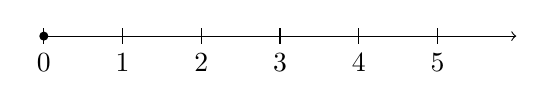
\begin{tikzpicture}
    \draw[->] (-3,0) -- (3,0); % node[right] {$x$};
    \foreach \x in {0,1,2,3,4,5}
    {
        \draw (\x-3,0.1) -- (\x-3,-0.1) node[below] {$\x$};
    }
    \draw[fill=black] (-3,0) circle (0.05); % origin
\end{tikzpicture}
\end{center}

\label{sec:zero-as-ordinal} \index{0!ordinal}
If number $a$ is on the left of number $b$, it means the order of $a$ is {\em before} $b$, or $a < b$, with distance of $b - a$; if $a$ is on the right of $b$, it means $a$ is {\em after} $b$, or $a > b$, with distance of $a - b$. We can combine this two cases by only defining $a < b$ as {\em before}, and negate it for the other. Alternatively, we may consider $a + d$ as to move $a$ forward (to the right) by $d$; $a - d$ to move backward (to the left) by $d$; if $d = 0$, then $a + 0 = a - 0 = a$, which {\em fixes} $a$. 0 has a valid order as those of 1, 2, 3, ..., but not a second class citizen.

\index{array}
Array is a data structure in computer system. It stores a collection of values in a consecutive cells in memory. For example,

\begin{lstlisting}[language=C, frame=single]
int a[10];
\end{lstlisting}

This line of code defines $a$ as an array, which stores 10 integers. Suppose an integer has 16 bits in the computer, the maximum integer is $2^{16}-1 = 65535$, which is $1111...1$ of sixteen 1s in binary; 314 is $100111010(=256 + 32 + 16 + 8 + 2)$ in binary, i.e., the bits at position 9, 6, 5, 4, 2 are 1, the other 11 positions are 0 (see \cref{sec:binary-numerals}). A byte has 8 bits, hence an integer of 16 bits occupies 2 bytes, or denoted as \lstinline|sizeof(int) = 2B = 16|. An array of 10 integers occupies $2 \times 10 = 20$ bytes in memory.

When executes the code \lstinline|int a[10]|, the computer will allocate 20 bytes in the memory\footnote{The are two types of memory: stack and heap; It is stack in this example.}, and point \lstinline|a| to the beginning position, called address. The program next uses this address to index an element of the array. The next two bytes from \lstinline|a| stores the first element; the 3rd and 4th bytes from \lstinline|a| stores the second element. The array stores 1, 2, ..., 9 as shown in \cref{fig:array}.

\begin{figure}[htbp]
 \centering
 \includegraphics[scale=0.35]{img/array}
 \caption{Array}
 \label{fig:array}
\end{figure}

Note the first element starts from \lstinline|a|. The distance between its address and \lstinline|a| is 0, denoted as \lstinline|a[0]|; The address of the next element starts from \lstinline|a + sizeof(int) = a + 16|, denoted as \lstinline|a[1]|; the next elements starts from \lstinline|a + 2 * sizeof(int)|, denoted as \footnote{`*' means multiplication}\lstinline|a[2]|... The computer indexes \lstinline|a[i]| at the position of \lstinline|a + i * sizeof(int)|. The 10 elements of the array are indexed as \lstinline|a[0], a[1], ..., a[9]|. This is the reason why array starts from 0 to $n - 1$ in programming: the index $i$ is the {\em distance} between element \lstinline|a[i]| and the starting address. Distance is from 0, the true starting point. Below example puts 1 to 10 into the array:

\begin{lstlisting}[language=C, frame=single]
int a[10];
for (int i = 0; i < 10; ++i) { a[i] = i + 1; }
\end{lstlisting}

There is a joke. A programmer treated his family to the restaurant after hard work of days and nights. He asked his kid how many meat balls in the dish. The kid pointed and counted 0, 1, 2, 3, ... Mom sighed he was born a programmer.

Many kids suffer from the `planting problems' in school. For example, (1) there are trees every 10 meters along a street of 100 meters long, how many trees in total? (2) There are trees every 20 meters around the playground of 400 meters long, how many trees in total? For problem (1), treat the street as the number line; start from 0, the 0th tree, the 1st tree, the 2nd tree, ..., the 10th tree. The distance between the $i$th tree and the starting point is $10i$ meters. As $100 \div 10 = 10$, the distance between the 10th tree and the starting point is 100 meters. 0, 1, 2, ..., 10, there are total 11 numbers, hence 11 trees. For problem (2), count from 0. As the circle (the shape of the playground) is 400 meters long, $400 \div 20 = 20$, the distance between the 20th tree and the starting point is 400 meters. The position of 20th tree overlaps with the 0th, hence is skipped. 0, 1, 2, ..., 19, $\cancel{20}$, there are total 20 trees. When shall we count from 1 and when count from 0? (see \cref{qn:count-from})

\subsection{Cardinal numbers}
\index{cardinal numbers}

It's incredible to change the view of zero from `nothingness' to `origin'. Different civilizations have diverse culture. The Genesis myth describes a state of chaos and nothingness before the world began, with heaven, earth, light, and beings marking the origin of the world. Buddhism holds the world we perceive is merely an illusion, the essence is nothingness. Ancient Chinese believed that yin and yang were the forces driving all changes, and that the vast universe emerged from the chaotic Tai Chi. With the integration of civilizations, the understanding of nothingness evolved. For example, Hegel started his logic with Being, Nothing, and Becoming (the quotation at the beginning of this chapter). According to the Big Bang theory, our universe originated from a massive explosion 13.8 billion years ago, there was no time or space prior to this event.

\index{empty set} \index{Frege}

If 0, as an ordinal number, is the starting point, can it become a cardinal number as the origin of beings? 3 as a cardinal number means there are three things, for example, 3cm: the length of 3 centimeters, 3g: the mass of 3 grams, 3 sheep, and so on; they are all three concrete things; The cardinal number 3 abstracts all collections of three things. In the language of set theory, it is a set of three elements, like $\{\bigstar, \square, \bigcirc \}$ or $\{a, b, c\}$. This is how logician Frege's definition of numbers. 0, which means nothing, is the cardinal number of the empty set (a set of nothing), denoted by $\varnothing$. This symbol was created by Bourbaki (a pen name of a group of anonymous mathematicians) in 1939. 1 is the cardinal number of a set of an element (a singleton) like $\{ \bigstar \}$, $\{ a \}$, or even $\{ \varnothing \}$. It is a set of set, containing the empty set as the only one element. The cardinal number of $\{ \varnothing \}$ is 1. As such, 1 arises from 0, nothing becomes being. We may go on constructing 2 from 1 by $\{ \varnothing, \{ \varnothing \} \}$. This set contains two distinct elements, both are sets: the empty set $\varnothing$ and $\{ \varnothing \}$. As 3 is the cardinal number of a set of three things, we then construct $\{ \varnothing, \{ \varnothing \}, \{ \varnothing, \{ \varnothing \} \}\}$, and so on.

\begin{tabular}{l|l}
  Cardinal number & set \\
  \hline
  0 & $\varnothing$ \\
  1 & $\{ \varnothing \}$ \\
  2 & $\{ \varnothing, \{ \varnothing \} \}$ \\
  3 & $\{ \varnothing, \{ \varnothing \}, \{ \varnothing, \{ \varnothing \} \}\}$ \\
  $\cdots$ & $\cdots$ \\
  $n$ & $\{ \varnothing, \{ \varnothing \}, \cdots \}$
\end{tabular}

Something is created from nothing. This table lists the steps from 0 to 1, to many.

\section{Negative numbers}
\index{negative numbers}

0 is the key to the magic box. Once is accepted, many questions arises: (1) 0 is prior to 1, what is prior to 0? (2) 1 is less than 2, 3, ... 0 is less than 1, what is less than 0? (3) What is the result of $a - b$ if $b > a$?

\index{The Nine Chapters on the Mathematical Art} \index{Liu Hui}
Although zero was accepted as a number around 1500 CE, the history of negative numbers is even shorter than zero. Most mathematicians in the 16th, 17th century rejected negative numbers\citepage[p208]{MKlein-1972}. Chinese was the earliest to adopt negative numbers. There was a classic book in Han Dynasty, named {\em The nine chapters on the mathematical art}, documented complete arithmetic rules for positive and negative numbers in the 8th chapter: {\em the method of positive and negative}. For example, `When subtracting numbers, subtract their values if both are positive or negative; add their values if they are opposite.' For addition, the rule was `add their values if both are positive or negative; subtract their values if they are opposite.' LIU Hui who was a mathematician of that time (flourished around 263 CE) later commented how to calculate with counting rods, `As the two numbers, one positive the other negative, offset each other, we need differentiate them with sign. Use the red rods for positive and the black for negative; alternatively (without using color), slant the rods to mark the number negative.'\cite{Jiuzhang-2009} (see \ref{sec:counting-rods} for counting rods). Chinese mathematician explained positive number as the income of sell, negative number as the cost of purchase. This is definitely a commercial application and it matched the traditional yin-yang culture. As shown in \cref{fig:yinyang}, yang is red for positive and yin is black for negative. Chinese people use yin and yang to denote negative and positive results of medical test and poles of electrodes.

\begin{figure}[htbp]
 \centering
 \includegraphics[scale=0.1]{img/yinyang}
 \caption{Yin and yang}
 \label{fig:yinyang}
\end{figure}

\index{Brahmagupta}

As Greeks viewed numbers as the magnitudes of geometric objects, like length, area, and volume, which were positive by nature. They needn't the notion of negative things. On top of the decimal positional system with zero, negative numbers appeared in India in the 7th century. Brahmagupta (589 - 670 CE, as \cref{fig:Brahmagupta}) clearly differentiated positive and negative numbers in his work. He interpreted them as fortunes and debts with dedicated sign to denote negative, then developed a set of calculation rules\cite{Rogers-2011}:

\begin{multicols}{2}
\begin{enumerate}[1)]
\item A debt minus zero is a debt.
\item A fortune minus zero is a fortune.
\item Zero minus zero is a zero.
\item A debt subtracted from zero is a fortune.
\item A fortune subtracted from zero is a debt.
\item The product of zero multiplied by a debt or fortune is zero.
\item The product of zero multiplied by zero is zero.
\item The product or quotient of two fortunes is one fortune.
\item The product or quotient of two debt is one fortune.
\item The product or quotient of a debt and a fortune is a debt.
\item The product or quotient of a fortune and a debt is a debt.
\end{enumerate}
\end{multicols}

\begin{figure}[htbp]
 \centering
 \includegraphics[scale=0.3]{img/Brahmagupta}
 \caption{Brahmagupta (by Andreas Strick)}
 \label{fig:Brahmagupta}
\end{figure}

\index{Diophantus}
Diophatus of Alexandria (200 - 284 CE) was the mathematician who studied the arithmetic independently of geometry. He was the first person known to use algebraic notation and symbolism that used an abridged notation for frequently occurring operations, and an abbreviation for the unknown and for the powers of the unknown. In his influential work {\em Arithmetica}, there was a problem to solve the equation $4 = 4x + 20$. As it led to negative solution, Diophantus thought it absurd. In the 9th century, Arabic mathematicians met negative numbers from the Indian works about mathematics and astronomy. However, they treated the negative inconsistently. For example, al-Khwarizmi allowed negative numbers when applying arithmetic rules to solve equations as they arose during moving or canceling terms; while he had to reject them in the final geometric argument. Al-Khwarizmi didn't generalize linear equations to $ax + b = 0$ or quadratic equations to $ax^2 + bx + c = 0$ as we see nowadays; to avoid negative coefficient, he categorized them into 6 types, such as $ax = b$, $b - ax = 0$, $ax^2 + bx = c$, $bx + c = ax^2$, $ax^2 + c = bx$. It was not until 15th century, did European mathematicians encounter negative numbers. Most people reject them. For example, when Girolamo Cardano (1501 - 1576) gave the methods of solution to the cubic and quartic equations in his {\em Ars Magma} (1545), he followed the tradition of Greeks, demonstrated with geometric argument. He interpreted the solution to linear equation as length, the solution to quadratic equation as area, and the solution to cubic equation as volume. Because of the rejection to the negative coefficient, Cardano had to list 60 types of equation.

\subsection{Ordinal numbers}
\index{John Wallis} \index{number line}
English mathematician John Wallis (1616 - 1703) introduced number line in the 17th century. It gave the ordinal meaning of negative numbers: they were numbers before zero, i.e., to the left of zero on the number line.

\begin{example}
In the dating system, 1 CE was the year after Jesus Christ's birth, then followed 2 CE, 3 CE, ... For the historic events happened before Jesus Christ's birth, we denote the year with BCE, for example, 1 BCE, 2 BCE, ... The years of BCE can be viewed as negative years (although lack of year 0).
\end{example}

\begin{example}
The temperature keeps decreasing in winter, finally to 3$\degree C$, 2$\degree C$, 1$\degree C$, 0$\degree C$, the freezing point. However, it's not the end; the temperature goes on decreasing below the freezing point. We see the red mark of thermometer (typically dyed alcohol with much lower freezing point than water) passes 0 degree, 1 degree below zero, 2 degrees below zero, ... the degrees below zero are negative.
\end{example}

Turn the thermometer horizontally and extend both sides infinitely, it becomes a number line:

\begin{center}
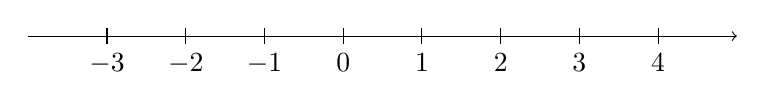
\begin{tikzpicture}
    \draw[->] (-4,0) -- (5,0);
    \foreach \x in {-3,-2,-1,0,1,2,3,4}
    {
        \draw (\x,0.1) -- (\x,-0.1) node[below] {$\x$};
    }
\end{tikzpicture}
\end{center}

Negative numbers and zero are to the left of positive numbers. Zero sits in the middle between the negative and positive numbers. The rules in \ref{sec:zero-as-ordinal} still hold: if $a < b$, then $a$ is to the left of $b$; if $b = 0$, then $a$ is negative; if $a = 0$, then $b$ is positive. From the perspective of ordering, the relation of `$<$' and `$>$' between two numbers correspond to the sign of their difference: if $a - b < 0$, then $a < b$, $a$ is to the left of $b$\footnote{Subtract $b$ from both sides of $a < b$ gives: $a - b < b - b = 0$}. If $a - b > 0$, then $a > b$, $a$ is to the right of $b$. For $d > 0$, $a + d$ advances (to the right) from $a$ by $d$; $a - d$ moves backward (to the left) by $d$; if $a < d$, then it moves to the range of negative numbers. For $d < 0$, it moves in opposite direction: $a + d$ moves backward (to the left), $a - d$ moves forward (to the right).

\subsection{Cardinal numbers}
\index{minus sign}
It looks strange to us that Wallis, the inventor of number line, thought negative numbers are greater than infinity, but not less than zero. In his \emph{Arithmetica Infinitorm} (1655) , Wallis explained: as the ratio $a/0$ is infinity\footnote{There was no rigors understanding to limit by the time of Wallis. As one of the pilots of Calculus, Wallis observed the ratio of $a/b$ increased very large for positive $a$ and $b$ when $b$ was close to 0. He, therefor, intuitively thought $a/0$ is infinity.} for positive $a$, therefore, when the denominator $b$ of $a/b$ further decreases to negative, the quotient will be greater than infinity\cite{MKlein-1972}.

People were generally confused about the cardinal meaning of negative numbers. Most mathematicians in the 16th, 17th century did not accept negative numbers as legitimate numbers and rejected them as `real roots' of equations\cite{MKlein-1972}. There was only a quadrant in Decartes's coordinate system; Pascal regarded the subtraction of 4 from 0 as utter nonsense. Tycho Brahe, the astronomer who used `-' as the minus sign, referred to negative numbers as "privative.
%% https://web.ma.utexas.edu/users/mks/326K/Negnos.html

\index{absolute value}
We can imagine how negative numbers confuses people. For example, Antarctica, with the temperature about 45 Celsius degrees below zero, is much colder than Helsinki, with the temperature about 10 degrees below zero in winter. If the magnitude shows how harsh the climate, then Antarctica should have a `larger' magnitude than Helsinki. However, $-45 < -10$ on the number line. Socrates (470 - 399 BCE) lived before Aristotle (384 - 322 BCE). In terms of the cardinal number, the years that Socrates lived should be `larger' than the years that Aristotle lived. However, $-470 < - 384$ on the number line. Such observation leads to the notion of {\em absolute value}. The absolute value of a number $a$ is the distance (length) between $a$ and 0 on the number line. It means the absolute value of a positive number is its value, for example the absolute value of 5 is $5 - 0 = 5$; the absolute value of a negative number is its opposite, for example, the absolute value of $-5$ is $0 - (-5) = 5$. 5 and $-5$ are bilateral symmetric to 0 on the number line, they are inverse of each other. The inverse of $a$ is $-a$. Because the distance between 0 to itself is $0 - 0 = 0$, the absolute value of 0 is 0. Denote the absolute value of $a$ by $|a|$, there are three cases:

\[
|a| = \begin{cases}
  a & a > 0 \\
  0 & a = 0 \\
  -a & a < 0
\end{cases}
\]

\index{van der Waerden} \index{pair} \label{sec:z-as-pair}
We may summarize them as: the absolute value of a positive number or zero is itself; the absolute value of a negative number is its inverse. In the influential text-book \emph{Modern Algebra} by Bartel Leendert van der Waerden\footnote{The textbook on abstract algebra is originally based on lectures given by Emil Artin in 1926 and by Emmy Noether from 1924 to 1928. The English translation of 1949 had the title \emph{Modern algebra}, though a later, extensively revised edition in 1970 had the title \emph{Algebra}.} there is a way to `constructed' integers, including negative numbers and zero, with a ordered pair of natural numbers $(a, b)$\citepage[p8]{van-der-Waerden-2009}.

\begin{itemize}
\item The pair $(a + b, b)$ corresponds to the positive number $a$.
\item The pair $(b, b)$ corresponds to 0.
\item The pair $(b, a + b)$ corresponds to the negative number $-a$.
\end{itemize}

For example, $(3, 1)$ corresponds to 2; $(5, 5)$ corresponds to 0; $(100, 101)$ corresponds to $-1$. For the ordered pair $(a, b)$, we may think about a balance with weights $a$ and $b$ on the two sides. When it balances, the weights of the pair $(b, b)$ are equal, their difference is 0; when the left weights more, the difference between the left and right is positive; when the right weights more, the difference is negative. There are multiple pairs corresponding to a number, for example: $(3, 1) = (9, 7) = (360, 358) = \cdots$ all correspond to 2; $(5, 5) = (100, 100) = (128, 128) = \cdots$ all correspond to 0; $(100, 101) = (1, 2) = (8, 9) = \cdots$ all correspond to $-1$. If treat them as equivalent classes, then each class of pair $(a, b)$ defines a distinct integer:

\begin{itemize}
\item If $a > b$, the pair defines the positive number $a - b$.
\item If $a = b$, the pair defines 0.
\item If $a < b$, the pair defines the negative number $-(b - a)$。
\end{itemize}

Define addition and multiplication for ordered pairs:

\begin{align}
(a, b) + (c, d) &= (a + c, b + d) \\
(a, b) \cdot (c, d) &= (ac + bd, ad + bc)
\label{eq:pair-add-mul}
\end{align}

For example of addition: $2 + (-1) = (5, 3) + (2, 3) = (7, 6) = 1$, multiplication: $-2 \times 3 = (1, 3) \cdot (5, 2) = (1 \times 5 + 3 \times 2, 1 \times 2 + 3 \times 5) = (11, 17) = -6$. \Cref{qn:pair-arithmetic} requires to verify the five arithmetic rules, i.e., associativity and commutativity of addition and multiplication, and the distribution of multiplication over addition, for ordered pairs.

This formal method defines positive numbers, zero, and negative numbers only with 1, 2, 3, ... bypasses all the questions to meanings of negative numbers and zero. As Leopold Kronecker said, \emph{God made the integers, all the rest is the work of man.}

\section{Number line}
With negative numbers and zero, the number line is marked with integers extend infinitely to both ends.

\begin{center}
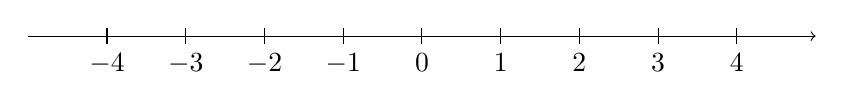
\begin{tikzpicture}
    \draw[->] (-5,0) -- (5,0);
    \foreach \x in {-4,-3,-2,-1,0,1,2,3,4}{
        \draw (\x,0.1) -- (\x,-0.1) node[below] {$\x$};
    }
\end{tikzpicture}
\end{center}

Here are some common notations: Denote natural numbers of 0, 1, 2, 3, ... by $\mathbb{N}$. Before 0 was accepted, natural numbers started from 1, 2, 3, ... people finally recognize 0 is the natural starting point, or origin (see \cref{sec:peano-axioms}); most authors define natural numbers starting from 0 nowadays. We often use $n$ to denote some natural number. The positive numbers, together with zero and negative numbers (e.g., $\dotsc, -3, -2, -1, 0, 1, 2, 3, \dotsc$) are integers, denoted by $\mathbb{Z}$. It comes from the initial letter of the German word `Zahlen' (meaning ``numbers''). We denote positive numbers by $\mathbb{Z}^+$ and negative numbers by $\mathbb{Z}^-$. We sometimes also use $i$ to denote some integer for it is the initial letter of the word `integer'. $i$ is more often used as the index to enumerate things, such as: $a_1, a_2, ..., a_i, ..., a_n$, where $a_i$ is the $i$-th element; $a_n$ is the $n$-th, which is commonly the last. Symbol matters in mathematics. The intuitive and vivid symbols are easy to understand with exceptional power, such as Leibniz's symbols for calculus. Vieta and Decartes were pioneers who used symbols systematically: they used $a, b, c$ to represent known quantities and $x, y, z$ to represent unknown quantities. These conventions have endured to the present.

\index{number line!arithmetic operations}
We can use number line to give intuitive meanings to the arithmetic operations ($+, -, \times, \div$), we'll give their geometric meanings in chapter 3. As mentioned in \cref{sec:zero-as-ordinal}, $a \pm b$ moves $a$ by $b$ units. There are five cases:

\begin{center}
  \begin{tabular}{c|c|c|c}
          & $b > 0$ & $b < 0$ & $b = 0$ \\
  \hline
  $a + b$ & move right     & move left    & \multirow{2}{*}{fix} \\
  \cline{1-3}
  $a - b$ & move left     & move right
  \end{tabular}
\end{center}

When $b < 0$, $a + b$ amounts to subtraction; $a - b$ amounts to add $a$ to $-b$. $b$ and $-b$ are additive inverse of each other, one may view subtraction as a special case of addition, thus to generalize above cases into three:

\begin{center}
\begin{tabular}{c|c|c|c}
        & $b > 0$ & $b < 0$ & $b = 0$ \\
\hline
$a + b$ & move right     & move left    & fix
\end{tabular}
\end{center}

\begin{figure}[htbp]
 \centering
 \includegraphics[scale=0.45]{img/translate}
\end{figure}

Give two numbers $a, b$ on the number line, their distance is:

\begin{center}
  \begin{tabular}{c|c|c|c}
      & $a < b$ & $a > b$ & $a = b$ \\
  \hline
  distance & $b - a$ & $a - b$ & $0$
  \end{tabular}
\end{center}

\begin{figure}[htbp]
 \centering
 \includegraphics[scale=0.4]{img/distance}
\end{figure}

This is the definition of absolute value, the distance is $|a - b|$. When $b = 0$, the distance of $a$ to the origin 0 is $|a|$.

\begin{figure}[htbp]
 \centering
 \includegraphics[scale=0.4]{img/abs}
\end{figure}

Distance as absolute value is non-negative, while difference between two numbers $a$ and $b$ on the number line, which is $a - b$ can be negative. If $a - b > 0$, then $a > b$, $a$ is to the right of $b$; if $a - b < 0$, then $a < b$, $a$ is to the left of $b$; if $a - b = 0$, then $a = b$, $a$ and $b$ coincide on the number line. Particularly, the difference between $a$ and the origin 0 is $a - 0 = a$, which equals to $a$ itself. The additive inverse of $a$ is the bilateral symmetric point $-a$ on the number line; the inverse of 0 is 0 itself.

\begin{center}
\begin{tikzpicture}
    \draw[->] (-3,0) -- (3,0);
    \draw (-2,0.1) -- (-2,-0.1) node [below] {$-a$};
    \draw (2,0.1) -- (2,-0.1)   node [below] {$a$};
    \draw (0,0.1) -- (0,-0.1)   node [below] {$0$};
\end{tikzpicture}
\end{center}

Here is how to make something out of nothing (0): $0 \begin{cases} n \\ -n \end{cases}$. 0 breaks into some $n$ and its inverse $-n$. Conversely, analogue to a pair of positron and electron, $n$ and $-n$ `annihilate' each other and produce 0. So far, we fix the number line and apply arithmetic operations to `move' points (numbers); as movement is relative, we may apply the operations to move the number line:

\subsection{Translation}
\index{number line!translation}
Which direction will the number line move if add $+1$ to {\em every} number on the number line? right or left? \cref{fig:plus-1-numline} shows the result:

\begin{figure}[htbp]
  \centering
  \begin{tikzpicture}{
      \draw[->] (-3,0) -- (4,0);
      \foreach \x in {-2,-1,0,1,2,3}{
          \draw (\x,0.1) -- (\x,-0.1) node[below] {$\x$};
      }
      \draw[fill=black] (0,0) circle (0.05); % origin

      \pgfmathsetmacro{\k}{-2}
      \draw[->] (-3,0+\k) -- (4,0+\k);
      \foreach \x in {-2,-1,0,1,2,3}{
          \pgfmathtruncatemacro{\y}{\x+1}
          \draw (\x,0.1+\k) -- (\x,-0.1+\k) node[below] {$\y$};
      }
      \draw[fill=black] (0-1,0+\k) circle (0.05); % origin
      \draw[->, decorate, decoration={snake, amplitude=.4mm, segment length=2mm, post length=1mm}]
        (0,0-0.8) -- (0,0+\k+0.3) node[above right] {$+1$};
  }
  \end{tikzpicture}
  \caption{Add $+1$ to every number on the number line.}
  \label{fig:plus-1-numline}
\end{figure}

Interestingly, it moves to the left by 1 unit. Adding 1 to each of $\{\cdots -2, -1, 0, 1, 2 \cdots \}$ gives $\{\cdots -1, 0, 1, 2, 3 \cdots \}$, indeed, it moves to the left by 1 unit. $-1$ is opposite to 1, thereby adding $-1$ moves the number line to the right, as shown in \cref{fig:minus-1-numline}.

\begin{figure}[htbp]
  \centering
  \begin{tikzpicture}{
      \draw[->] (-3,0) -- (4,0);
      \foreach \x in {-2,-1,0,1,2,3}{
          \draw (\x,0.1) -- (\x,-0.1) node[below] {$\x$};
      }
      \draw[fill=black] (0,0) circle (0.05); % origin

      \pgfmathsetmacro{\k}{-2}
      \draw[->] (-3,0+\k) -- (4,0+\k);
      \foreach \x in {-2,-1,0,1,2,3}{
          \pgfmathtruncatemacro{\y}{\x-1}
          \draw (\x,0.1+\k) -- (\x,-0.1+\k) node[below] {$\y$};
      }
      \draw[fill=black] (0-1,0+\k) circle (0.05); % origin
      \draw[->, decorate, decoration={snake, amplitude=.4mm, segment length=2mm, post length=1mm}]
        (0,0-0.8) -- (0,0+\k+0.3) node[above right] {$-1$};
  }
  \end{tikzpicture}
  \caption{Add$-1$ to every number on the number line.}
  \label{fig:minus-1-numline}
\end{figure}

In general, adding $+a$ moves the number line by $-a$; adding $-a$ moves the number line by $a$.

\begin{center}
  \begin{tabular}{c|c|c|c}
                   & $a > 0$ & $a < 0$ & $a = 0$ \\
  \hline
  $\mathbb{Z} + a$ & move left     & move right    & \multirow{2}{*}{fix} \\
  \cline{1-3}
  $\mathbb{Z} - a$ & move right     & move left
  \end{tabular}
\end{center}

Why does the number line move inversely with $a$? Denote the number line before moving by $A$, after moving by $A'$. Every number $x$ on $A$ is sent to $x \rightsquigarrow x + a$, which is $x' = x + a$ on $A'$. In particular, $-a$ on $A$ is sent to $-a \rightsquigarrow -a + a = 0$, which is the origin on $A'$. The origin on number line $A'$ {\em corresponds} to the point of $-a$ on the number line $A$. If $a > 0$, then the new origin (corresponding to $-a$) is to the left of the old origin, as shown in \cref{fig:translate-number-line}.

\begin{figure}[htpb]
  \centering
  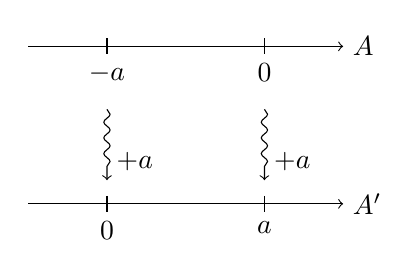
\begin{tikzpicture}{
      \draw[->] (-3,0) -- (1,0) node[right] {$A$};
      \draw (-2,0.1) -- (-2,-0.1) node[below] {$-a$};
      \draw (0, 0.1) -- (0, -0.1) node[below] {$0$};

      \pgfmathsetmacro{\k}{-2}
      \draw[->] (-3,0+\k) -- (1,0+\k) node[right] {$A'$};
      \draw (-2,0.1+\k) -- (-2,-0.1+\k) node[below] {$0$};
      \draw (0, 0.1+\k) -- (0, -0.1+\k) node[below] {$a$};

      \draw[->, decorate, decoration={snake, amplitude=.4mm, segment length=2mm, post length=1mm}]
          (-2,0-0.8) -- (-2,0+\k+0.3) node[above right] {$+a$};
      \draw[->, decorate, decoration={snake, amplitude=.4mm, segment length=2mm, post length=1mm}]
          (0,0-0.8) -- (0,0+\k+0.3) node[above right] {$+a$};
}
  \end{tikzpicture}
  \caption{Translation of number line}
  \label{fig:translate-number-line}
\end{figure}

\subsection{Inverse}
\index{additive inverse} \index{number line!inverse}
When negate every number, the number line is inverse (rotate $180\degree$ against the origin).

\begin{figure}[htpb]
  \centering
  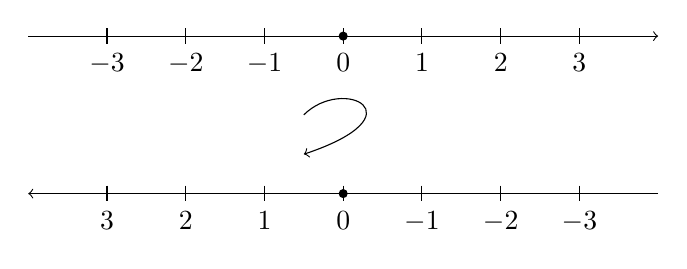
\begin{tikzpicture}{
      \draw[->] (-4,0) -- (4,0);
      \foreach \x in {-3,-2,-1,0,1,2,3}{
          \draw (\x,0.1) -- (\x,-0.1) node[below] {$\x$};
      }
      \draw[fill=black] (0,0) circle (0.05); % origin

      \pgfmathsetmacro{\k}{-2}
      \draw[->] (4,0+\k) -- (-4,0+\k);
      \foreach \x in {-3,-2,-1,0,1,2,3}{
          \pgfmathtruncatemacro{\y}{-\x}
          \draw (\x,0.1+\k) -- (\x,-0.1+\k) node[below] {$\y$};
      }
      \draw[fill=black] (0,0+\k) circle (0.05); % origin
      \draw[->] (-0.5, -1) .. controls (0, -0.5) and (1, -1.0) .. (-0.5, -1.5);
  }
  \end{tikzpicture}
  \caption{Inverse of number line.}
  \label{fig:negate-number-line}
\end{figure}

The number line restores when negating twice; rotate $180\degree$, then rotate $180\degree$ again, it is equivalent to rotate $360\degree$, and is equivalent to fix.

\btab{ccccc}
  $\rightarrow$ & invert & $\leftarrow$ & invert & $\rightarrow$ \\
\hline
  $a$           & negate & $-a$       & negate & $-(-a) = a$
\etab

The effect of negating a number $a \rightsquigarrow -a$ amounts to multiplying it by $-1$, as $-a = a (-1) = (-1) a$. Negating twice restores a number explains why negative times negative is positive: $-(-a) = (-1)(-a) = a$.

\subsection{Scale}
\index{number line!scale}
Multiplication means scaling (\cref{sec:mul-as-zoom}). $\times 2$ scale up the number line two times; $\times 3$ scale up three times; $\div 2$ scale down the number line to $\frac{1}{2}$; $\div 3$ scale down to $\frac{1}{3}$. Division is multiplicative inverse; thus $\div 2$ amounts to $\times \frac{1}{2}$, which scales down to $\frac{1}{2}$; $\div 3$ scale down to $\frac{1}{3}$. In this way, we may generalize division as multiplication:

\begin{center}
  \begin{tabular}{c|c|c|c}
             & $a > 1$ & $0 < a < 1$ & $a = 1$ \\
  \hline
  $\times a$ & scale up     & scale down    & fix \\
  \end{tabular}
\end{center}

The scaling factor can be negative. As mentioned above, $\times (-1)$ amounts to negating, which inverses the number line; $\times (-2)$ amounts to scaling up 2 times followed by inverting: $(-1) \times 2$; it also amounts to inverting followed by scaling up 2 times: $2 \times (-1) = (-1) \times 2$. $\times (-3)$ amounts to scaling up 3 times followed by inverting, or inverting followed by scaling up 3 times. Below table generalizes multiplication and division:

\begin{center}
  \begin{tabular}{c|c|c|c|c|c|c}
             & $a > 1$ & $a = 1$ & $0 < a < 1$  & $-1 < a < 0$ & $a = -1$ & $a < -1$ \\
  \hline
  $\times a$ & scale up     & fix    & scale down          & scale down + invert & invert & scale up + invert
  \end{tabular}
\end{center}

There is a special case: when $\times 0$, the number line collapses into a point. The operations can be composed: translation of $a$ followed by translation of $b$ amounts to translation of $b$ followed by translation of $a$; that $a + b = b + a$ is the commutative law of addition. Scaling with $a$ followed by scaling with $b$ amounts to scaling with $b$ followed by scaling with $a$; that $ab = ba$ is the commutative law of multiplication. We leave the explanation of the association law with number line as \cref{qn:assiciative-numline}.

There are complex composition such as translation followed by scaling or inverting, for example, $x \rightsquigarrow ax + b$ which scaling with $a$ followed by translation of $-b$. \Cref{qn:transform-numline} applies translation followed by scaling.

\section{Unit}
\index{unit} \label{sec:unit}
0 and negative numbers are the first class citizen as those of 1, 2, 3, ... they have ordinal meaning (the valid and definitive position on the number line) and  cardinal meaning (the valid and definitive value). 0 is special; it is the origin, the staring point, the symbol of nothing. Is there any other number as special as 0? Below table compares 1 with 0:

\begin{align*}
  0     &             &  1 & \\
  1 + 0 & = 0 + 1 = 1  &  1 \times 0 &= 0 \times 1 = 0 \\
  2 + 0 &= 0 + 2 = 2  &  1 \times 2  &= 2 \times 1 = 2 \\
  3 + 0 &= 0 + 3 = 3  &  1 \times 3  &= 3 \times 1 = 3 \\
  \cdots &            & \cdots & \\
  a + 0 &= 0 + a = a  &  1 \times a  &= a \times 1 =  a
\end{align*}

Adding 0 to any number leaves that number unchanged; multiplying any number (including 0) by 1 leaves that number unchanged. Let us see the effective of 0 and 1 to the number line:

\begin{enumerate}[1)]
\item Addition moves the number line to the left or right. $+a$ moves the number line by $-a$ (moves left when $a > 0$; moves right when $a < 0$), 0 fixes the number line under addition.
\item Multiplication scales up or down the number line. $\times a$ scales the number line $a$ times (scale up when $|a| > 1$; scale down when $0 < |a| < 1$), 1 fixes the number line under multiplication.
\end{enumerate}

For any number $a$, there is one and only one additive symmetric number to 0, which is its inverse, $-a$, satisfying $a + (-a) = 0$. For any number $a \ne 0$, there is one and only one multiplicative symmetric number to 1, which is its reciprocal, $\frac{1}{a}$, satisfying $a \times \frac{1}{a} = 1$. But 0 does not have reciprocal. Which one is more special, 0 or 1?

There are plenty of things behaving like 0 and 1. For example, we call a sequence of characters a string. Word, phrases, sentences are strings, hence ``apple'', ``hello'', ``to be or not to be'', `` '' (a space) are all strings. One can concatenate strings, like ``hello'' $\doubleplus$ `` '' = ``hello '', ``hello '' $\doubleplus$ ``apple'' = ``hello apple''. A string that doesn't contain any character is empty, namely the empty string ``''. Concatenating any string with the empty string leaves that string unchanged:

\[
\text{``''} \doubleplus S = S \doubleplus \text{``''} = S
\]

For example, ``'' $\doubleplus$ ``hello'' = ``hello'' $\doubleplus$ ``'' = ``hello''. Define the union of two sets is a set that contains all distinct elements from the two, for example $\{a, b, c\} \cup \{1, 2, 3\} = \{a, b, c, 1, 2, 3\}$, $\{a, b, c\} \cup \{c, d, e\} = \{a, b, c, d, e\}$. Taking the union of any set with the empty set $\varnothing$ leaves that set unchanged:

\[
\varnothing \cup S = S \cup \varnothing = S
\]

For example, $\varnothing \cup \{a, b, c\} = \{a, b, c\} \cup \varnothing = \{a, b, c\}$. In mathematics, 0 is the unit under addition; 1 is the unit under multiplication; the empty string ``'' is the unit under string concatenation; the empty set $\varnothing$ is the unit under set union. In general, if there is some element $e$ in set $M$ (can be finite or infinite), under the binary operation $\odot$ satisfying:

\[
  e \odot a = a \odot e = a
\]

for any element $a$ of $M$, then $e$ is a unit of $M$ under $\odot$. We may check with this definition that, 0 is a unit under addition in the set of numbers; 1 is a unit under multiplication in the set of numbers excluding 0; empty string is a unit under concatenation in the set of strings; empty set is a unit under union in the \emph{set of sets}. A unit is a first class citizen as other elements in the set, and it is special and unique (see \cref{qn:unique-e}). For this reason, we call it {\em the} unit.

\index{inverse}
For element $a$ in a set, if there is some element $b$ in that set satisfying $a \odot b = e$, then we call $b$ the inverse of $a$. For example, the additive inverse of any number $a$ is $-a$ because $a + (-a) = 0$; the multiplicative inverse of any non-zero number $a$ is $\frac{1}{a}$ because $a \times \frac{1}{a} = 1$. Inverse does not always exist necessarily, for example, strings don't have inverse under concatenation except for the empty string; sets don't have inverse under union except for the empty set. Inverse enables us to simplify four arithmetic operations ($+, -, \times, \div$) to two: $a - b$ is $a$ plus the additive inverse of $b$, $a \div b$ is $a$ times the multiplicative inverse of $b$ (the reciprocal).

\section{Peano's axioms}
\label{sec:peano-axioms}
Giuseppe Peano, an Italian mathematician, established an axiomatic system for natural numbers in 1889. His started from zero, and applied counting operation to cover natural numbers. There are five axioms:

\index{Peano's axioms}
\begin{enumerate}[{Axiom} 1)]
\item 0 is a natural number.
\item (counting) For every natural number $n$, there is a successor $n'$.
\end{enumerate}

It seems one can define infinitely many natural numbers with these two axioms; from 0, the next is 1, followed by 2, 3, ..., $n$, and $n + 1$, ... However, here is a counter example: a set of two numbers $\{0, 1\}$. Define 1 as the successor of 0, while 0 as the successor of 1. It well satisfies the above two axioms although unexpected. We need the third axiom to exclude this situation.

\begin{enumerate}[{Axiom} 1)]
  \setcounter{enumi}{2}
  \item 0 is not the successor of any natural number.
\end{enumerate}

However, it's still not enough. For another counter example: a set of $\{0, 1, 2\}$. Define 1 as the successor of 0, 2 as the successor of 1, and 2 as the successor of 2 itself. It satisfies all the three axioms. We need the fourth:

\begin{enumerate}[{Axiom} 1)]
  \setcounter{enumi}{3}
  \item The successors are distinct. If $m$ and $n$ have the same successor, then they are identical, i.e. $m = n$ if and only if $m' = n'$.
\end{enumerate}

Hold on, it is still insufficient. For another counter example: set \{0, 0.5, 1, 1.5, 2, 2.5, ...\}. Define 1 as the successor of 0, 2 as the successor of 1... define 1.5 as the successor of 0.5, 2.5 as the successor of 1.5... But 0.5 is not the successor of any number. We need the last axiom to exclude such `unreachable' elements.

\begin{enumerate}[{Axiom} 1)]
  \setcounter{enumi}{4}
  \item If some subset $S$ of natural numbers contains 0, and every element in $S$ has a successor, then $S$ is $\mathbb{N}$.
\end{enumerate}

\index{axiom of induction} \index{mathematical induction}
Why does the fifth axiom exclude the counter example of \{0, 0.5, 1, 1.5, 2, 2.5, ...\}? Consider its strict subset of \{0, 1, 2, ...\}. 0 belongs to it, and every element has a successor, but it is not identical to the original set. As 1.5, 2.5, ... are not in this subset, it does not satisfy the fifth axiom. The last axiom is also known as the {\em axiom of induction}, which is often stated equivalently as below.

\begin{enumerate}[{Axiom} 1)]
  \setcounter{enumi}{4}
  \item For any proposition regarding to natural numbers, if it is true for 0, and whenever being true for some number $n$, it is also true for $n'$ (the successor), then the proposition is true for all natural numbers. (This axiom ensures the correctness of mathematical induction.)
\end{enumerate}

To show we can reach the top floor of a skyscraper by mathematical induction, we take two steps: 1) show we can enter the lobby of the building; 2) show at any floor we can always step upstairs to the next floor. These are Peano's five axioms, which form the axiomatic system known as Peano's arithmetic. We next show how arithmetic operations are defined in this system. The definition of addition consists of two parts: adding 0 to any natural number leaves  the number unchanged; and $a$ plus the successor of $b$ equals to the successor of the sum of $a$ and $b$. \index{natural numbers!addition}

\be
\begin{laligned}
a + 0  &= a \\
a + b' &= (a + b)'
\end{laligned}
\label{eq:peano-add}
\ee

Let us verify $2+3$ with this definition. 2 is the successor of the successor of 0, denoted by $0''$; 3 is the successor of the successor of the successor of 0, denoted by $0''$. The sum of $2 + 3$ by this definition is:

\[
0'' + 0''' = (0'' + 0'')' = (0'' + 0')'' = (0'' + 0)''' = (0'')''' = 0'''''
\]

Indeed, it is the five times successor of 0, which is 5. We may understand this definition with number line: to move from $a$ on the number line to the right by $b'$, one first move by $b$ and then move by 1. Such kind of definition that includes a definition of itself is called {\em recursive}. It breaks down a problem into some same smaller problems. In the definition of addition, the original problem of $a + b'$ is {\em recursively} converted to the problem of $a + b$, which reduces the `level' of the complexity by 1. If $b \ne 0$, then continuously reducing the complexity; if $b = 0$, then the recursion terminates at $a + 0 = a$. Here 0 is called the exit of the recursion. We next define multiplication for natural numbers:\index{natural numbers!multiplication}

\be
\begin{laligned}
a \cdot 0 &= 0 \\
a \cdot b' &= a \cdot b + a
\end{laligned}
\label{eq:peano-multiply}
\ee

The definition of multiplication consists of two parts: the product of any natural number and 0 is 0, and the product of $a$ and the successor of $b$ equals to adding $a$ to the product of $a$ and $b$. The latter can be expressed as $a \cdot (b+1) = a \cdot b + a \cdot 1$. Let's verify it with $2 \times 3$:

\begin{align*}
0'' \times 0''' & = 0'' \times 0'' + 0'' = 0'' \times 0' + 0'' + 0'' = 0'' \times 0 + 0'' + 0'' + 0'' \\
                & = 0 + 0'' + 0'' + 0'' = 0'' + 0'' + 0'' = (0'' + 0')' + 0'' = (0'' + 0)'' + 0'' \\
                & = (0'')'' + 0'' = 0'''' + 0'' \\
                & = (0'''' + 0')' = (0'''' + 0)'' = (0'''')'' = 0''''''
\end{align*}

Indeed, it's the six times successor of 0, which is 6. The definition of multiplication is recursive too; it breaks down the problem of calculating $a \cdot b'$ into two sub-problems: (1) recursively calculate $a \cdot b$ (reduce the level of complexity by 1); (2) add $a$ to the result of the first problem. The recursion terminates when $b$ decreases to 0. The idea of the recursive method is `divide and conquer'; it is powerful and widely used, particularly in the modern computer system.

\index{associativity of addition} \label{sec:add-assoc}
It turns out that neither the associativity nor the commutativity of addition or multiplication is axiom. One can prove them all with Peano's axioms. For example, to prove $(a + b) + c= a + (b + c)$, the associativity of addition by induction, first, we show it holds when $c=0$. According to the first rule of addition:

\[
(a + b) + 0 = a + b = a + (b + 0)
\]

Second, assume $(a + b) + c = a + (b + c)$ holds, we are going to show $(a + b) + c' = a + (b + c')$.

\begin{align*}
(a + b) + c' &= (a + b + c)' && \text{2nd rule of +, (converse)} \\
             &= (a + (b + c))' && \text{induction assumption} \\
             &= a + (b + c)' && \text{2nd rule of +} \\
             &= a + (b + c') && \text{2nd rule of +, (converse)} & \mbox{\qed}
\end{align*}

It proves the associativity of addition. However, it is a bit complex to prove the commutativity of addition; \cref{app:add-commutativity} gives a proof.

\begin{mdframed}
\index{Peano}

\begin{center}
 \includegraphics[scale=0.2]{img/Peano}
 \captionof{figure}{Giuseppe Peano, 1858-1932}
 \label{fig:Peano}
\end{center}

Giuseppe Peano was an mathematician, logician, and linguist. He was born and raised on a farm at Spinetta, a hamlet now belonging to Cuneo, Italy. He entered the University of Turin in 1876, graduating in 1880 with high honors, after which the University employed him to teach calculus course. In 1887, Peano married Carola Crosio. In 1886, he began teaching concurrently at the Royal Military Academy. From 1880s, Peano started to study mathematical logic. He published Peano's axioms, a formal foundation for the natural numbers in 1889. Peano started the \emph{Formulario} Project. It was to be an `Encyclopedia of Mathematics', containing all known formulae and theorems. In 1900, the Second International Congress of Mathematicians was held in Paris. At the conference Peano met Bertrand Russell and gave him a copy of \emph{Formulario}. Russell was so struck by Peano's innovative logical symbols that he left the conference and returned home to study Peano's text\cite{M-Kline-2007}.

When Russell and Whitehead wrote {\em Principia Mathematica}, they were deeply influenced by Peano. Peano played a key role in the axiomatization of mathematics and was a leading pioneer in the development of mathematical logic and set theory. As part of this effort, he made key contributions to the modern rigorous and systematic treatment of the method of mathematical induction. He spent most of his career teaching mathematics at the University of Turin. He also developed an international auxiliary language, Latino sine flexione (`Latin without inflections', later called Interlingua), which is a simplified version of classical Latin. Although Peano put a lot of effort to rewrite his works in the new language, few people read it. On the other hand, his early works in French influenced many mathematicians, especially to Bourbaki school. Peano died on April 20th, 1932.
\end{mdframed}

\begin{Exercise}[label={ex:zero}]
\Question{Peoples of different civilizations independently developed the notion of area when measuring lands, and connected it with multiplication as shown in \cref{fig:rectangle-vanish}. When the width is 0, the area of $0 \times 5$ disappears. What shape does the rectangle become?

  \begin{center}
  \includegraphics[scale=0.3]{img/rectangles}
  \captionof{figure}{The rectangle of $0 \times 5$ disappears.}
  \label{fig:rectangle-vanish}
  \end{center}
}
\Question{When shall we count from 1? when shall we count from 0? \label{qn:count-from}}
\Question{*Define subtraction and division for pairs.}
\Question{Verify the addition and multiplication of pairs are commutative, associative, and the multiplication is distributive over addition.\label{qn:pair-arithmetic}}
\Question{Show that $(-1) \times (-1) = 1$ by the distributive law.}
\Question{Show that the additive inverse is unique.}
\Question{Use the number line to explain the meaning of the associative law of addition and multiplication.\label{qn:assiciative-numline}}
\Question{To implement the transformation of $x \rightsquigarrow 2x + 1$ by translation followed by scaling, which direction need move? and how far? after that, how big need scale? In general, how to implement the transformation of $x \rightsquigarrow ax + b$? \label{qn:transform-numline}}
\Question{Show that a unit is unique. \label{qn:unique-e}}
\Question{*Define 1 as the successor of 0, show that $a \cdot 1 = a$ for any natural number $a$. Hint: use the result of \cref{app:add-commutativity}.}
\Question{*Prove the distributive property of multiplication by Peano's axioms.}
\Question{*Prove the associativity and commutativity of multiplication by Peano's axioms.}
\Question{*How to verify $3 + 147 = 150$ by Peano's axiom?}
\end{Exercise}

\begin{Answer}[ref={ex:zero}]
\Question{View the area of rectangle as multiplication. When the width is 0, the area of $0 \times 5$ disappears. What shape does the rectangle become?

\vspace{2mm}
On one hand, consider the width keeps decreasing; the rectangle is narrowing and is closing to a line segment with length of 5. By Euclid's definition: line has no width. The dimension of width disappears, leaving only one dimension of height. On the other hand, point has no size by Euclid; no length or width, which corresponds to $0 \times 0$.
}

\Question{When shall we count from 1? when shall we count from 0?

\vspace{2mm}
We need consider if it regards ordinal meaning or cardinal meaning; whether regards the notion of distance (from the origin), whether accepts negative value, and so on.
}

\Question{Define subtraction and division for pairs.

  \begin{enumerate}[(a)]
  \item Subtraction amounts to adding the inverse. The inverse of $(a, b)$ is $(b, a)$. Define: $(a, b) - (c, d) = (a, b) + (d, c) = (a + d, b + c)$.
  \item To define division, note two things: (1) $(ka, kb)$ amounts to scaling up $(a, b)$ by $k$ times; $(\frac{1}{k}a, \frac{1}{k}b)$ amounts to scaling down to $\frac{1}{k}$. (2) $(-a, -b) = (b, a)$; from where gives below definition:

    \[
    (a, b) / (c, d) = \begin{dcases}
        c > d: & (\dfrac{a}{c-d}, \dfrac{b}{c-d}) \\
        c < d: & (\dfrac{b}{d-c}, \dfrac{a}{d-c})
        \end{dcases}
    \]
    where $c \ne d$。
  \end{enumerate}
}

\Question{Verify the addition and multiplication of pairs are commutative, associative, and the multiplication is distributive over addition.

  \begin{enumerate}[(a)]
  \item Commutative:
    \begin{align*}
      (a, b) + (c, d) & = (a + c, b + d)  & \text{sum of pairs} \\
                      & = (c + a, d + b)  & \text{commutative of + for } \mathbb{N}\\
                      & = (c, d) + (a, b) & \text{sum of pairs (converse)}
    \end{align*}
    \begin{align*}
      (a, b) \cdot (c, d) & = (ac + bd, ad + bc) & \text{product of pairs} \\
                          & = (ca + db, da + cb) & \text{commutative of . for } \mathbb{N} \\
                          & = (c, d) \cdot (a, b) & \text{product of pairs (converse)}
    \end{align*}
  \item We skip for associativity
  \item There are two distributive law: from left and from right. We only verify the left one.
    \begin{align*}
         &(a, b) \cdot ((c, d) + (e, f)) & \\
        =& (a, b) \cdot (c + e, d + f) & \\
        =& (a(c + e) + b (d + f), a(d + f) + b(c + e)) & \\
        =& (ac + bd + ae + bf, ad + bc + af + be) & \\
        =& (ac + bd, ad + bc) + (ae + bf, af + be) & \text{sum of pairs (converse)} \\
        =& (a, b) \cdot (c, d) + (a, b) \cdot (e, f) & \text{product of pairs (converse)}
    \end{align*}
  \end{enumerate}
}

\Question{Show that $(-1) \times (-1) = 1$ by the distributive law.
  \begin{proof}
    \begin{align*}
      (-1) \times (-1) & = (-1) \times (-1) + 0 & \text{fixed when } + 0 \\
                      & = (-1) \times (-1) + (-1 + 1) & \text{additive inverse} \\
                      & = (-1) \times (-1) + (-1) \times 1 + 1 & \text{fixed when } \times 1\\
                      & = (-1) \times (-1 + 1) + 1 & \text{distributive law (converse)} \\
                      & = (-1) \times 0 + 1 = 0 + 1 = 1 & \qedhere
    \end{align*}
  \end{proof}
}

\Question{Show that the additive inverse is unique.
  \begin{proof}
    Suppose $b$ is another additive inverse of $a$, we are going to show $b = -a$:
    \begin{align*}
      0     & = b + a     & \text{additive inverse} \\
      0 - a & = b + a - a & -a \text{ on both sides} \\
      -a & = b + (a - a)  = b + 0 = b & \qedhere
    \end{align*}
  \end{proof}
}

\Question{Use the number line to explain the meaning of the associative law of addition and multiplication.

\vspace{2mm}
Addition: The move of the number line, that first moves $a + b$ followed by another move of $c$, which amounts to first moves $a$ followed by another move of $b + c$. Multiplication: first scale up the number line $ab$ times followed by another scaling of $c$; it amounts to first scale up $a$ followed by another scaling of $bc$.
}

\Question{To implement the transformation of $x \rightsquigarrow 2x + 1$ by translation followed by scaling, which direction need move? and how far? after that, how big need scale? In general, how to implement the transformation of $x \rightsquigarrow ax + b$?

\vspace{2mm}
Since $2x + 1 = 2(x + \frac{1}{2})$, the transformation is to first move {\em left} by $\frac{1}{2}$ followed by scaling up 2 times. In general, as $ax + b = a(x + \frac{b}{a})$, the transformation is to move by $-\frac{b}{a}$ (move left if $\frac{b}{a}>0$, otherwise move right), followed by scaling $a$ times.
}

\Question{Show that a unit is unique.
\begin{proof}
Suppose there is another unit $e'$, which satisfies $e' \odot a = a \odot e' = a$ for any element $a$. We are going to show $e = e'$:
\begin{align*}
e &= e \odot e' & e'\text{ is a unit} & \\
  &= e'         & e\text{ is a unit}  &\qedhere
\end{align*}
\end{proof}
}

\Question{Define 1 as the successor of 0, show that $a \cdot 1 = a$ for any natural number $a$.

\begin{proof}
Using the result in \cref{app:add-commutativity}: $0 + a = a$,

\begin{align*}
a' \cdot 1 & = a' \cdot 0' && \text{1 is the successor of 0} \\
           & = a' \cdot 0 + a' && \text{2nd rule of multiplication} \\
           & = 0 + a' && \text{1st rule of multiplication} \\
           & = a' && \qedhere
\end{align*}

\end{proof}
}
\Question{Prove the distributive property of multiplication by Peano's axioms.

\begin{proof}
We only prove the left distributive law: $c(a + b) = ca + cb$. By induction on $b$, when $b = 0$:

\begin{align*}
c(a + 0) & = ca && \text{1st rule of addition} \\
         & = ca + 0 && \text{1st rule of addition (converse)} \\
         & = ca + c0 && \text{1st rule of multiplication (converse)}
\end{align*}

Assume $c(a + b) = ca + cb$ holds, we are going to show $c(a + b') = ca + cb'$:

\begin{align*}
c(a + b') & = c(a + b)' & \text{2nd rule of addition} & \\
          & = c(a + b) + c & \text{2nd rule of multiplication} &\\
          & = ca + cb + c & \text{induction assumption} &\\
          & = ca + (cb + c) & \text{associativity of addition} &\\
          & = ca + cb' & \text{2nd rule of multiplication (converse)} & \qedhere
\end{align*}
\end{proof}
}
\Question{Prove the associativity and commutativity of multiplication by Peano's axioms.

\begin{proof}
We only prove the associative law: $(ab)c = a(bc)$ and outline the scheme to prove the commutative law. By induction on $c$, when $c = 0$:

\begin{align*}
(ab)0 & = 0 && \text{1st rule of multiplication} \\
      & = a0 && \text{1st rule of multiplication (converse)} \\
      & = a(b0) && \text{1st rule of multiplication (converse)}
\end{align*}

Assume $(ab)c = a(bc)$, we are going to show $(ab)c' = a(bc')$:

\begin{align*}
(ab)c' & = (ab)c + ab & \text{2nd rule of multiplication} &\\
       & = a(bc) + ab & \text{induction assumption} &\\
       & = a(bc + b) & \text{distributive law (previous exercise)} &\\
       & = a(bc') & \text{2nd rule of multiplication} &\qedhere
\end{align*}
\end{proof}

One may prove the commutative law for multiplication in three steps, each with induction: (1) show $1a = a$; (2) prove the right distributive law: $(a + b)c = ac + bc$; (3) prove the commutative law finally.
}

\Question{How to verify $3 + 147 = 150$ by Peano's axiom?

\vspace{3mm}
Here is the classic proof to $2 + 2 = 4$:

\begin{align*}
2 + 2 &=  0'' + 0'' && \text{each is the twice successor of 0} \\
      &=  (0'' + 0')' && \text{2nd rule of addition} \\
      &=  ((0'' + 0)')' && \text{2nd rule of addition} \\
      &=  ((0'')')' && \text{1st rule of addition} \\
      &=  0'''' = 4 && \text{four times successor of 0}
\end{align*}

It would be too long to show $3 + 147 = 150$ in this way. We may apply the commutative law (in previous exercise) first, convert it to an easier one: $147 + 3 = 150$; alternatively, we show $3 + a = a'''$ by induction.
}
\end{Answer}

\ifx\wholebook\relax \else
\section{Answer}
\shipoutAnswer

\section{Commutativity of addition}
\subimport{inc/}{addcom-en}

\begin{thebibliography}{99}
\subimport{inc/}{bib-en}
\end{thebibliography}

\expandafter\enddocument
\fi
